\documentclass[12pt]{article}
\usepackage[a4paper, total={6in, 10in}]{geometry}
\usepackage{graphicx}
\graphicspath{{figs/}} 


\title{
Analysis of Movement Variability for Facial Expressions 
with Nonlinear Dynamics
} 
\author{Miguel Xochicale\\ 
}
\date{21th December 2018}

\begin{document}
\maketitle
%\thispagestyle{empty} %No number


%\begin{abstract}
%
%\end{abstract}


\section{Introduction}
Movement variability is an inherent feature within and between persons. 
Research on measurement and understanding of movement variability has been 
well established in the last three decades in areas such as biomechanics, 
sport science, psychology, cognitive science, neuroscience and robotics 
\cite{XochicalePhDThesis2018}
With that in mind, I hypothesise that the subtle variations of facial 
expressions can be quantified in a similar fashion as with the methodologies 
of movement variability. Hence, I am interested in quantifying the complexity 
of facial expression that one person or multiple can present in scenarios 
of human-robot interaction, particularly I am interested in these two questions: 
(i) can the quantification of the variation of facial expressions tell us 
something about the state of health or the state of mind of a person?, 
(ii) how the quantification of facial expressions can be related with 
the complexity of the facial expressions?.


\section{Methods}
Considering my work of my PhD thesis for quantification of movement variability 
using nonlinear dynamics methods \cite{2018arXiv181009249X},
I am proposing to work with Recurrence Quantification Analysis (RQA). 
RQA computes measurements based on the recurrence points density of diagonal 
or vertical line structures in Recurrence Plots. 
Such measurements of dynamics can determine the determinism (predictability) 
or Shannon entropy (complexity) of a nonlinear system \cite{marwan2007}. 
Hence, I am proposing to use Shannon Entropy measurement 
from the recurrent quantification analysis, also known as RQAEntr 
to quantify the complexity of face expressions. 
(Fig \ref{fig:method}).


%%---------------------------------(FIGURE)-------------------------------------
\begin{figure}
\centering
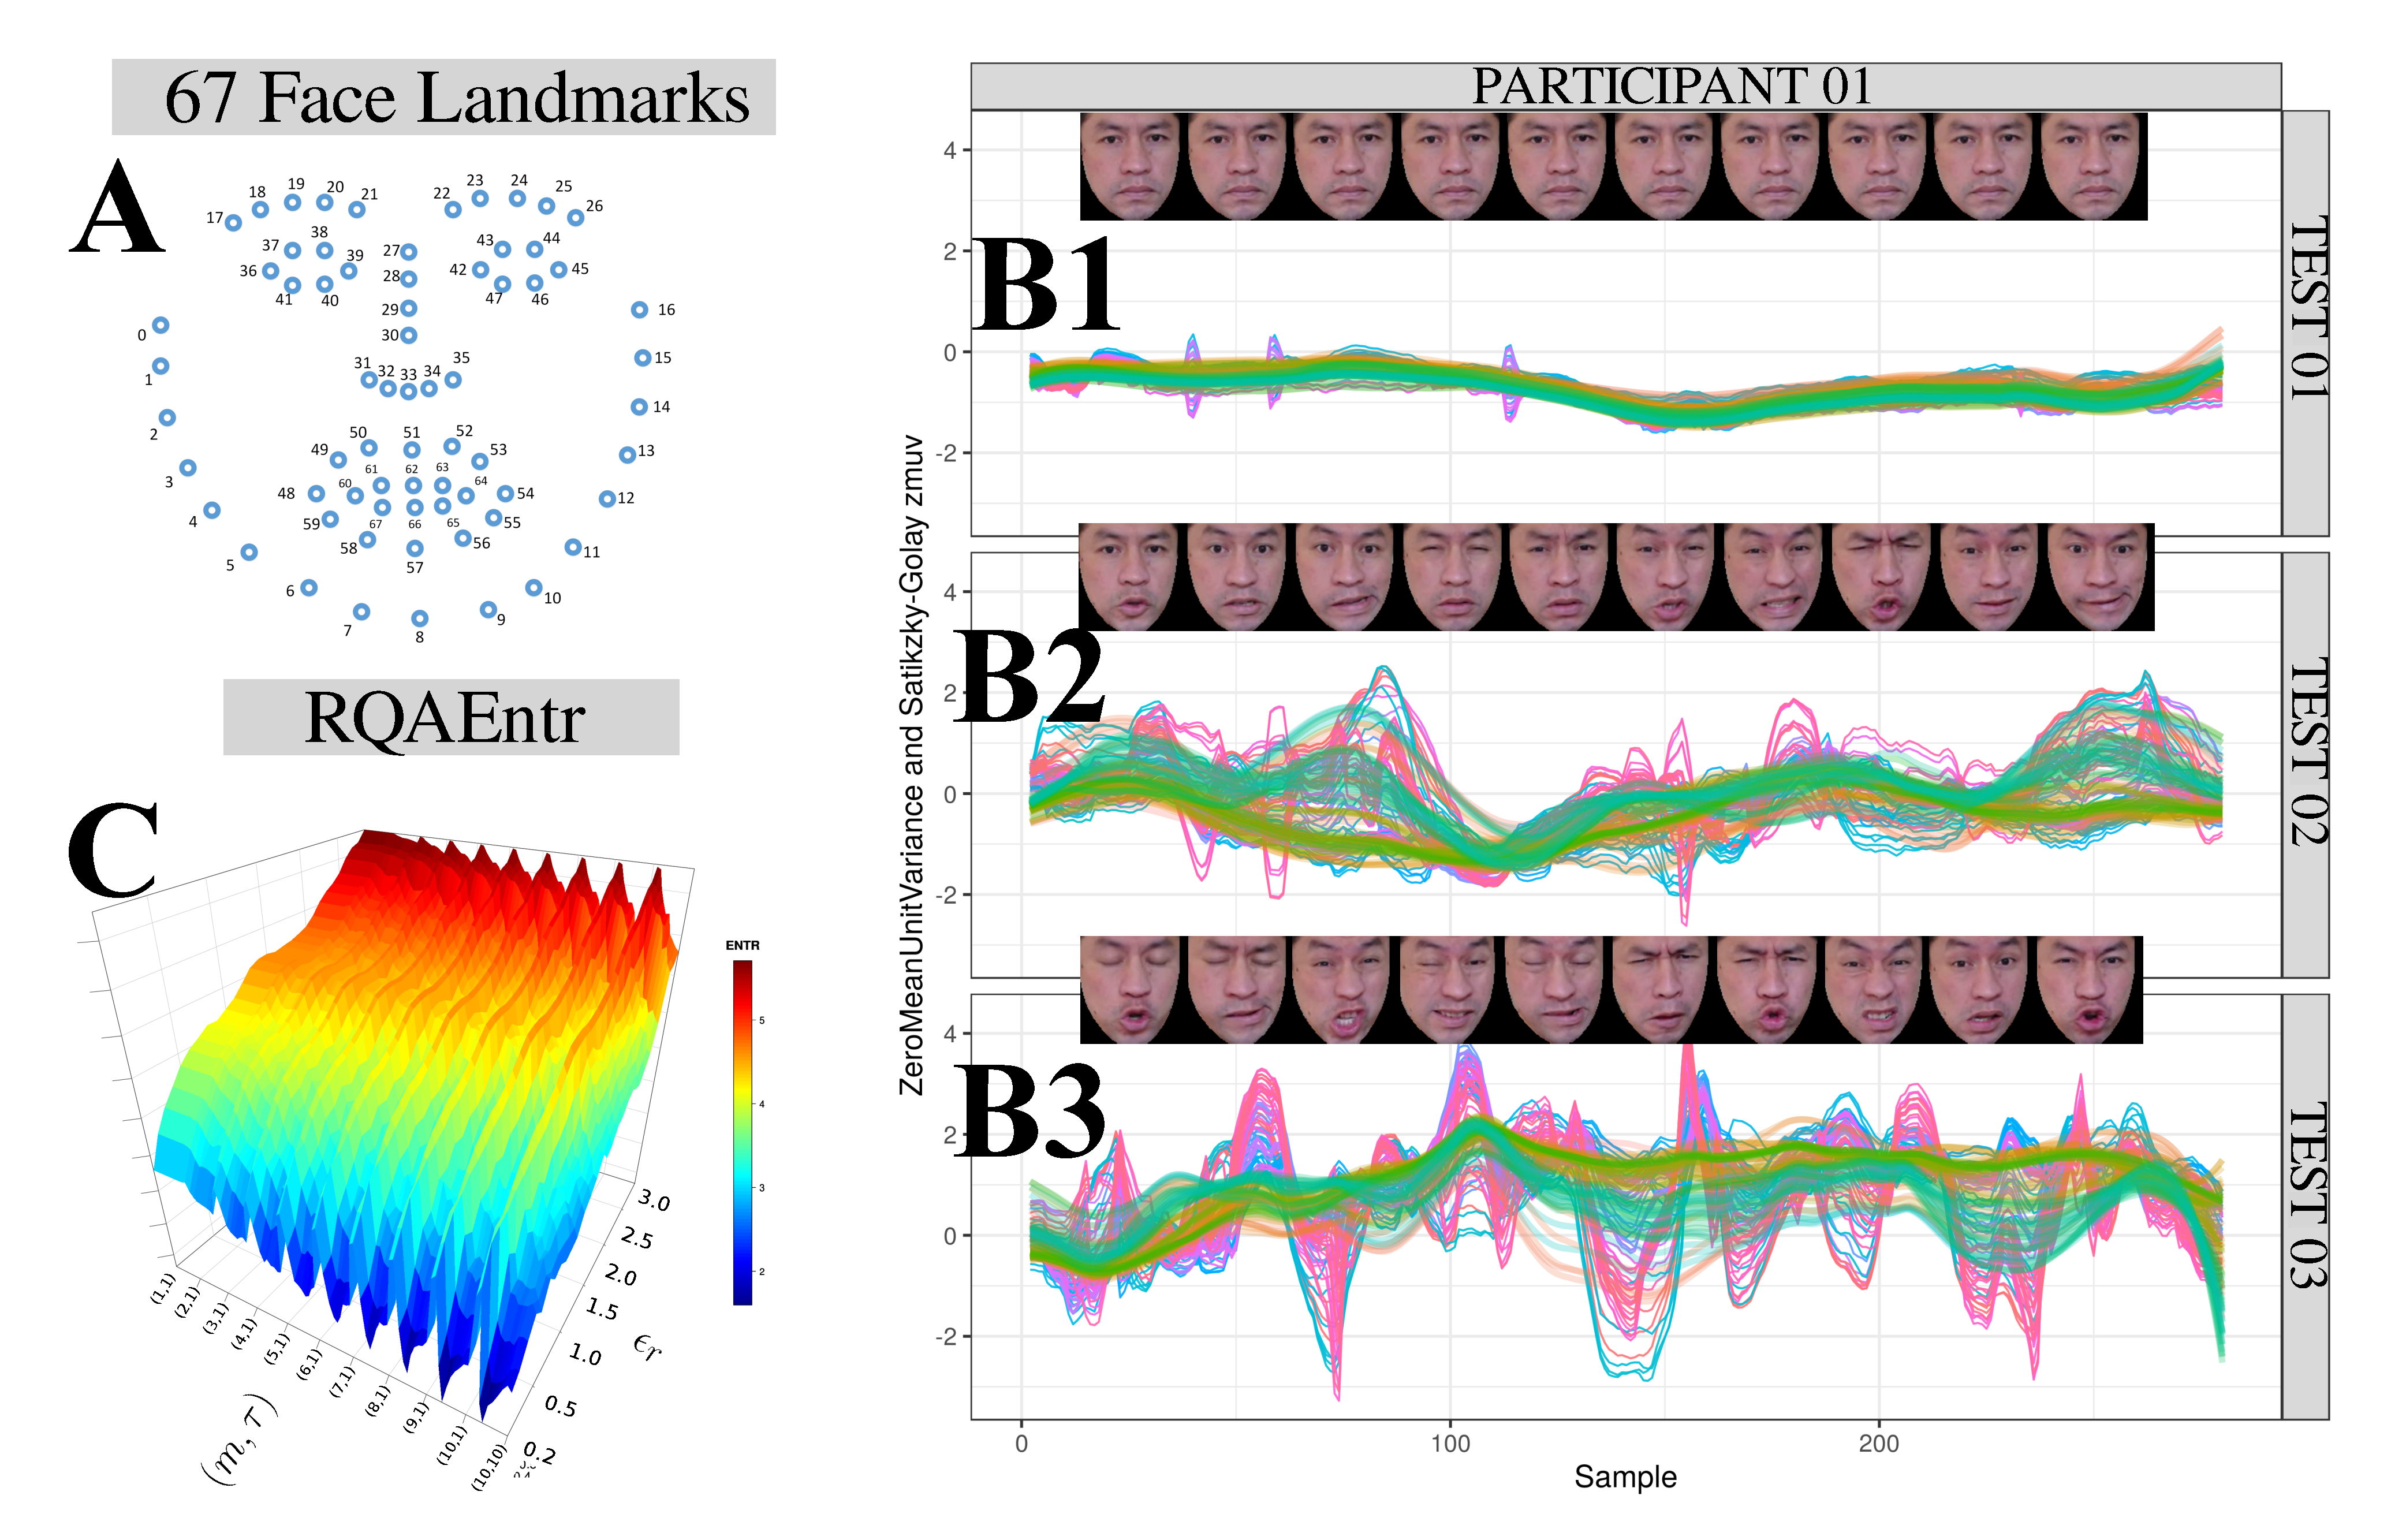
\includegraphics[width=1.0\textwidth]{main/method}
    \caption{
	{\bf Quantifying variations of face variations using nonlinear dynamics.}
	(A) Head pose estimation and face landmarks with OpenFace \cite{baltrusaitis2018},
	(B) time series from landmarks, and
	(C) 3D surface of RQAEntr for one time series.
        }
\label{fig:method}
\end{figure}
%%---------------------------------(FIGURE)------





%\newpage

\bibliographystyle{apalike}
\bibliography{references/references}


\end{document}
